% Copyright (c) 2022-2026 MKM Research Labs. Licensed under the MIT License; see LICENSE.
%
% Gauge calibration to observed river levels -- the change document for the v2.0.0
% releases of the gauge-response, gauge-history and GEV hazard-curve models. Filed on
% each of those models as Core Documentation. Its tables are generated from the data by
% tools/gauge_calibration/tables.py into evidence_tables.tex.
%
% Build: pdflatex three times in this folder (the third settles "Page n of N").
\documentclass[11pt,a4paper]{article}
\newcommand{\doctitle}{Gauge Calibration to Observed River Levels}
\newcommand{\docsubtitle}{Rating-curve shape match of the Thames gauges to Environment Agency records}
\newcommand{\docversion}{1.0}
\newcommand{\docdate}{07-November-2026}
\newcommand{\docauthor}{David K Kelly}
% MKM Research Labs — Shared Document Header
% Usage: % MKM Research Labs — Shared Document Header
% Usage: % MKM Research Labs — Shared Document Header
% Usage: \input{../shared/mkm_header}  (before \begin{document})
%
% Required commands before \input:
%   \newcommand{\doctitle}{...}
%   \newcommand{\docsubtitle}{...}
%   \newcommand{\docversion}{1.0}
%   \newcommand{\docdate}{13-February-2026}
%   \newcommand{\docauthor}{David K Kelly}

% ─── Packages ───────────────────────────────────────────────────────────────
\usepackage[utf8]{inputenc}
\usepackage{amsmath,amsfonts,amssymb}
\usepackage{listings}
\usepackage{color,xcolor}
\usepackage{graphicx}
\usepackage{hyperref}
\usepackage[toc,page]{appendix}
\usepackage{tabto}
\usepackage{float}
\usepackage{comment}
\usepackage[en-GB]{datetime2}
\usepackage{setspace}
\usepackage{subcaption}
\usepackage{booktabs}
\usepackage{longtable}
\usepackage{adjustbox}
\usepackage{enumitem}
\usepackage{fancyhdr}
\usepackage{lastpage}

% ─── Page geometry ──────────────────────────────────────────────────────────
\onehalfspacing
\usepackage{geometry}
\geometry{a4paper, total={170mm,247mm}, left=20mm, top=25mm, bottom=25mm}

% ─── Headers and footers ───────────────────────────────────────────────────
\pagestyle{fancy}
\fancyhf{}
\fancyhead[L]{\small\textcolor{gray}{MKM Research Labs}}
\fancyhead[R]{\small\textcolor{gray}{\doctitle{} --- v\docversion}}
\fancyfoot[C]{\small\textcolor{gray}{CONFIDENTIAL}}
\fancyfoot[R]{\small\textcolor{gray}{Page \thepage\ of \pageref{LastPage}}}
\renewcommand{\headrulewidth}{0.4pt}
\renewcommand{\footrulewidth}{0.4pt}

% ─── Colours ────────────────────────────────────────────────────────────────
\definecolor{mkmblue}{HTML}{1565C0}
\definecolor{codegreen}{rgb}{0,0.6,0}
\definecolor{codegray}{rgb}{0.5,0.5,0.5}
\definecolor{codepurple}{rgb}{0.58,0,0.82}
\definecolor{backcolour}{rgb}{0.95,0.95,0.92}

% ─── Hyperref setup ─────────────────────────────────────────────────────────
\hypersetup{
    colorlinks=true,
    linkcolor=mkmblue,
    citecolor=mkmblue,
    urlcolor=mkmblue
}

% ─── Code listings ──────────────────────────────────────────────────────────
\lstdefinestyle{mystyle}{
    backgroundcolor=\color{backcolour},
    commentstyle=\color{codegreen},
    keywordstyle=\color{magenta},
    numberstyle=\tiny\color{codegray},
    stringstyle=\color{codepurple},
    basicstyle=\ttfamily\footnotesize,
    breakatwhitespace=false,
    breaklines=true,
    captionpos=b,
    keepspaces=true,
    numbers=left,
    numbersep=5pt,
    showspaces=false,
    showstringspaces=false,
    showtabs=false,
    tabsize=2
}
\lstset{style=mystyle}

% ─── Section formatting ────────────────────────────────────────────────────
\setcounter{tocdepth}{3}
\setcounter{secnumdepth}{3}

% ─── Shared macros ──────────────────────────────────────────────────────────
\newcommand{\mkmtitlepage}{%
    \begin{titlepage}
    \begin{center}
    \vspace*{1cm}
    \begin{figure}[H]\centering
        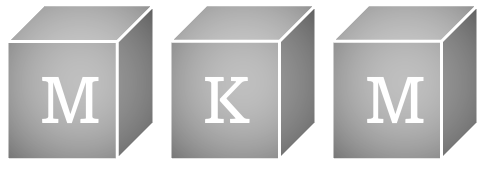
\includegraphics[width=0.4\textwidth]{../shared/Logos/MKM_logo.png}
    \end{figure}
    \vspace{1.5cm}
    {\Huge\bfseries\textcolor{mkmblue}{\doctitle}\par}
    \vspace{0.5cm}
    {\Large\textcolor{gray}{\docsubtitle}\par}
    \vspace{2cm}
    {\large MKM Research Labs\par}
    \vspace{0.5cm}
    {\large Version \docversion{} --- \docdate\par}
    \vspace{0.5cm}
    {\large \docauthor\par}
    \vspace{2cm}
    \textcolor{red}{\textbf{CONFIDENTIAL --- PROPRIETARY}}
    \end{center}
    \end{titlepage}
}

\newcommand{\mkmlegalpage}{%
    \clearpage
    \thispagestyle{empty}
    \begin{center}
    \large\textbf{Legal Notice}
    \vspace{1em}

    \textbf{PROPRIETARY AND CONFIDENTIAL}
    \end{center}

    \noindent This document, including all algorithms, models, methodology, formulas,
    calculations, and intellectual concepts contained herein, constitutes the exclusive
    intellectual property and confidential trade secrets of MKM Research Labs (``MKM'').

    \vspace{0.5em}
    \noindent Any usage, reproduction, distribution, modification, or disclosure of this
    document or any portion thereof, without the express prior written authorisation from
    MKM Research Labs is strictly prohibited and constitutes an infringement of intellectual
    property rights.

    \vspace{0.5em}
    \noindent The document is provided on an ``as is'' basis. MKM Research Labs makes no
    representations or warranties of any kind, express or implied, regarding its accuracy,
    reliability, or suitability for any particular purpose.

    \vspace{1em}
    \begin{center}
    All rights reserved. \copyright\ 2021--2026 MKM Research Labs.

    \vspace{0.5em}
    Governed by the laws of the United Kingdom.
    \end{center}
    \clearpage
}

\newcommand{\mkmhistorypage}[1]{%
    \section{Document History}
    \begin{table}[ht]
        \centering
        \begin{tabular}{l|l|l|l}
            \textbf{Date} & \textbf{Version} & \textbf{Description} & \textbf{Author} \\
            \hline
            #1
        \end{tabular}
        \label{tab:revision_history}
    \end{table}
    \clearpage
}

% ─── Bank validation protocol section commands ──────────────────────────────
% Use these to ensure every model doc has the required sections.
% They are just styled \section calls — content is provided by each doc.

\newcommand{\mkmexecsummary}{\section{Executive Summary}}
\newcommand{\mkmpurpose}{\section{Model Purpose and Scope}}
\newcommand{\mkmframework}{\section{Mathematical Framework}}
\newcommand{\mkminputs}{\section{Input Parameters and Calibration}}
\newcommand{\mkmimplementation}{\section{Implementation Details}}
\newcommand{\mkmsensitivity}{\section{Sensitivity Analysis}}
\newcommand{\mkmvalidation}{\section{Validation and Backtesting}}
\newcommand{\mkmtestresults}{\subsection{Automated Test Results}\input{test_results}}
\newcommand{\mkmlimitations}{\section{Model Limitations and Known Weaknesses}}

\newcommand{\mkmgovernance}{\section{Governance Validation Questions}
\noindent The following nine questions are mandated by Chapter~5 of the
\emph{Model Risk Governance for Vendors} handbook and must be explicitly
addressed for every model in the inventory. Response status is tracked in the
Model Governance Dashboard (MRC portal). \par\medskip}

\newcommand{\mkmvqitem}[3]{\subsection{Q#1 --- #2}
\noindent\textit{``#3''}\par\medskip\noindent}

\newcommand{\mkmchangelog}{\section{Change History}}
  (before \begin{document})
%
% Required commands before \input:
%   \newcommand{\doctitle}{...}
%   \newcommand{\docsubtitle}{...}
%   \newcommand{\docversion}{1.0}
%   \newcommand{\docdate}{13-February-2026}
%   \newcommand{\docauthor}{David K Kelly}

% ─── Packages ───────────────────────────────────────────────────────────────
\usepackage[utf8]{inputenc}
\usepackage{amsmath,amsfonts,amssymb}
\usepackage{listings}
\usepackage{color,xcolor}
\usepackage{graphicx}
\usepackage{hyperref}
\usepackage[toc,page]{appendix}
\usepackage{tabto}
\usepackage{float}
\usepackage{comment}
\usepackage[en-GB]{datetime2}
\usepackage{setspace}
\usepackage{subcaption}
\usepackage{booktabs}
\usepackage{longtable}
\usepackage{adjustbox}
\usepackage{enumitem}
\usepackage{fancyhdr}
\usepackage{lastpage}

% ─── Page geometry ──────────────────────────────────────────────────────────
\onehalfspacing
\usepackage{geometry}
\geometry{a4paper, total={170mm,247mm}, left=20mm, top=25mm, bottom=25mm}

% ─── Headers and footers ───────────────────────────────────────────────────
\pagestyle{fancy}
\fancyhf{}
\fancyhead[L]{\small\textcolor{gray}{MKM Research Labs}}
\fancyhead[R]{\small\textcolor{gray}{\doctitle{} --- v\docversion}}
\fancyfoot[C]{\small\textcolor{gray}{CONFIDENTIAL}}
\fancyfoot[R]{\small\textcolor{gray}{Page \thepage\ of \pageref{LastPage}}}
\renewcommand{\headrulewidth}{0.4pt}
\renewcommand{\footrulewidth}{0.4pt}

% ─── Colours ────────────────────────────────────────────────────────────────
\definecolor{mkmblue}{HTML}{1565C0}
\definecolor{codegreen}{rgb}{0,0.6,0}
\definecolor{codegray}{rgb}{0.5,0.5,0.5}
\definecolor{codepurple}{rgb}{0.58,0,0.82}
\definecolor{backcolour}{rgb}{0.95,0.95,0.92}

% ─── Hyperref setup ─────────────────────────────────────────────────────────
\hypersetup{
    colorlinks=true,
    linkcolor=mkmblue,
    citecolor=mkmblue,
    urlcolor=mkmblue
}

% ─── Code listings ──────────────────────────────────────────────────────────
\lstdefinestyle{mystyle}{
    backgroundcolor=\color{backcolour},
    commentstyle=\color{codegreen},
    keywordstyle=\color{magenta},
    numberstyle=\tiny\color{codegray},
    stringstyle=\color{codepurple},
    basicstyle=\ttfamily\footnotesize,
    breakatwhitespace=false,
    breaklines=true,
    captionpos=b,
    keepspaces=true,
    numbers=left,
    numbersep=5pt,
    showspaces=false,
    showstringspaces=false,
    showtabs=false,
    tabsize=2
}
\lstset{style=mystyle}

% ─── Section formatting ────────────────────────────────────────────────────
\setcounter{tocdepth}{3}
\setcounter{secnumdepth}{3}

% ─── Shared macros ──────────────────────────────────────────────────────────
\newcommand{\mkmtitlepage}{%
    \begin{titlepage}
    \begin{center}
    \vspace*{1cm}
    \begin{figure}[H]\centering
        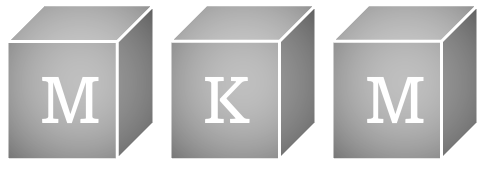
\includegraphics[width=0.4\textwidth]{../shared/Logos/MKM_logo.png}
    \end{figure}
    \vspace{1.5cm}
    {\Huge\bfseries\textcolor{mkmblue}{\doctitle}\par}
    \vspace{0.5cm}
    {\Large\textcolor{gray}{\docsubtitle}\par}
    \vspace{2cm}
    {\large MKM Research Labs\par}
    \vspace{0.5cm}
    {\large Version \docversion{} --- \docdate\par}
    \vspace{0.5cm}
    {\large \docauthor\par}
    \vspace{2cm}
    \textcolor{red}{\textbf{CONFIDENTIAL --- PROPRIETARY}}
    \end{center}
    \end{titlepage}
}

\newcommand{\mkmlegalpage}{%
    \clearpage
    \thispagestyle{empty}
    \begin{center}
    \large\textbf{Legal Notice}
    \vspace{1em}

    \textbf{PROPRIETARY AND CONFIDENTIAL}
    \end{center}

    \noindent This document, including all algorithms, models, methodology, formulas,
    calculations, and intellectual concepts contained herein, constitutes the exclusive
    intellectual property and confidential trade secrets of MKM Research Labs (``MKM'').

    \vspace{0.5em}
    \noindent Any usage, reproduction, distribution, modification, or disclosure of this
    document or any portion thereof, without the express prior written authorisation from
    MKM Research Labs is strictly prohibited and constitutes an infringement of intellectual
    property rights.

    \vspace{0.5em}
    \noindent The document is provided on an ``as is'' basis. MKM Research Labs makes no
    representations or warranties of any kind, express or implied, regarding its accuracy,
    reliability, or suitability for any particular purpose.

    \vspace{1em}
    \begin{center}
    All rights reserved. \copyright\ 2021--2026 MKM Research Labs.

    \vspace{0.5em}
    Governed by the laws of the United Kingdom.
    \end{center}
    \clearpage
}

\newcommand{\mkmhistorypage}[1]{%
    \section{Document History}
    \begin{table}[ht]
        \centering
        \begin{tabular}{l|l|l|l}
            \textbf{Date} & \textbf{Version} & \textbf{Description} & \textbf{Author} \\
            \hline
            #1
        \end{tabular}
        \label{tab:revision_history}
    \end{table}
    \clearpage
}

% ─── Bank validation protocol section commands ──────────────────────────────
% Use these to ensure every model doc has the required sections.
% They are just styled \section calls — content is provided by each doc.

\newcommand{\mkmexecsummary}{\section{Executive Summary}}
\newcommand{\mkmpurpose}{\section{Model Purpose and Scope}}
\newcommand{\mkmframework}{\section{Mathematical Framework}}
\newcommand{\mkminputs}{\section{Input Parameters and Calibration}}
\newcommand{\mkmimplementation}{\section{Implementation Details}}
\newcommand{\mkmsensitivity}{\section{Sensitivity Analysis}}
\newcommand{\mkmvalidation}{\section{Validation and Backtesting}}
\newcommand{\mkmtestresults}{\subsection{Automated Test Results}\input{test_results}}
\newcommand{\mkmlimitations}{\section{Model Limitations and Known Weaknesses}}

\newcommand{\mkmgovernance}{\section{Governance Validation Questions}
\noindent The following nine questions are mandated by Chapter~5 of the
\emph{Model Risk Governance for Vendors} handbook and must be explicitly
addressed for every model in the inventory. Response status is tracked in the
Model Governance Dashboard (MRC portal). \par\medskip}

\newcommand{\mkmvqitem}[3]{\subsection{Q#1 --- #2}
\noindent\textit{``#3''}\par\medskip\noindent}

\newcommand{\mkmchangelog}{\section{Change History}}
  (before \begin{document})
%
% Required commands before \input:
%   \newcommand{\doctitle}{...}
%   \newcommand{\docsubtitle}{...}
%   \newcommand{\docversion}{1.0}
%   \newcommand{\docdate}{13-February-2026}
%   \newcommand{\docauthor}{David K Kelly}

% ─── Packages ───────────────────────────────────────────────────────────────
\usepackage[utf8]{inputenc}
\usepackage{amsmath,amsfonts,amssymb}
\usepackage{listings}
\usepackage{color,xcolor}
\usepackage{graphicx}
\usepackage{hyperref}
\usepackage[toc,page]{appendix}
\usepackage{tabto}
\usepackage{float}
\usepackage{comment}
\usepackage[en-GB]{datetime2}
\usepackage{setspace}
\usepackage{subcaption}
\usepackage{booktabs}
\usepackage{longtable}
\usepackage{adjustbox}
\usepackage{enumitem}
\usepackage{fancyhdr}
\usepackage{lastpage}

% ─── Page geometry ──────────────────────────────────────────────────────────
\onehalfspacing
\usepackage{geometry}
\geometry{a4paper, total={170mm,247mm}, left=20mm, top=25mm, bottom=25mm}

% ─── Headers and footers ───────────────────────────────────────────────────
\pagestyle{fancy}
\fancyhf{}
\fancyhead[L]{\small\textcolor{gray}{MKM Research Labs}}
\fancyhead[R]{\small\textcolor{gray}{\doctitle{} --- v\docversion}}
\fancyfoot[C]{\small\textcolor{gray}{CONFIDENTIAL}}
\fancyfoot[R]{\small\textcolor{gray}{Page \thepage\ of \pageref{LastPage}}}
\renewcommand{\headrulewidth}{0.4pt}
\renewcommand{\footrulewidth}{0.4pt}

% ─── Colours ────────────────────────────────────────────────────────────────
\definecolor{mkmblue}{HTML}{1565C0}
\definecolor{codegreen}{rgb}{0,0.6,0}
\definecolor{codegray}{rgb}{0.5,0.5,0.5}
\definecolor{codepurple}{rgb}{0.58,0,0.82}
\definecolor{backcolour}{rgb}{0.95,0.95,0.92}

% ─── Hyperref setup ─────────────────────────────────────────────────────────
\hypersetup{
    colorlinks=true,
    linkcolor=mkmblue,
    citecolor=mkmblue,
    urlcolor=mkmblue
}

% ─── Code listings ──────────────────────────────────────────────────────────
\lstdefinestyle{mystyle}{
    backgroundcolor=\color{backcolour},
    commentstyle=\color{codegreen},
    keywordstyle=\color{magenta},
    numberstyle=\tiny\color{codegray},
    stringstyle=\color{codepurple},
    basicstyle=\ttfamily\footnotesize,
    breakatwhitespace=false,
    breaklines=true,
    captionpos=b,
    keepspaces=true,
    numbers=left,
    numbersep=5pt,
    showspaces=false,
    showstringspaces=false,
    showtabs=false,
    tabsize=2
}
\lstset{style=mystyle}

% ─── Section formatting ────────────────────────────────────────────────────
\setcounter{tocdepth}{3}
\setcounter{secnumdepth}{3}

% ─── Shared macros ──────────────────────────────────────────────────────────
\newcommand{\mkmtitlepage}{%
    \begin{titlepage}
    \begin{center}
    \vspace*{1cm}
    \begin{figure}[H]\centering
        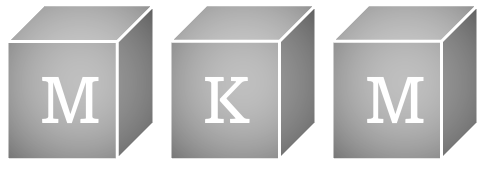
\includegraphics[width=0.4\textwidth]{../shared/Logos/MKM_logo.png}
    \end{figure}
    \vspace{1.5cm}
    {\Huge\bfseries\textcolor{mkmblue}{\doctitle}\par}
    \vspace{0.5cm}
    {\Large\textcolor{gray}{\docsubtitle}\par}
    \vspace{2cm}
    {\large MKM Research Labs\par}
    \vspace{0.5cm}
    {\large Version \docversion{} --- \docdate\par}
    \vspace{0.5cm}
    {\large \docauthor\par}
    \vspace{2cm}
    \textcolor{red}{\textbf{CONFIDENTIAL --- PROPRIETARY}}
    \end{center}
    \end{titlepage}
}

\newcommand{\mkmlegalpage}{%
    \clearpage
    \thispagestyle{empty}
    \begin{center}
    \large\textbf{Legal Notice}
    \vspace{1em}

    \textbf{PROPRIETARY AND CONFIDENTIAL}
    \end{center}

    \noindent This document, including all algorithms, models, methodology, formulas,
    calculations, and intellectual concepts contained herein, constitutes the exclusive
    intellectual property and confidential trade secrets of MKM Research Labs (``MKM'').

    \vspace{0.5em}
    \noindent Any usage, reproduction, distribution, modification, or disclosure of this
    document or any portion thereof, without the express prior written authorisation from
    MKM Research Labs is strictly prohibited and constitutes an infringement of intellectual
    property rights.

    \vspace{0.5em}
    \noindent The document is provided on an ``as is'' basis. MKM Research Labs makes no
    representations or warranties of any kind, express or implied, regarding its accuracy,
    reliability, or suitability for any particular purpose.

    \vspace{1em}
    \begin{center}
    All rights reserved. \copyright\ 2021--2026 MKM Research Labs.

    \vspace{0.5em}
    Governed by the laws of the United Kingdom.
    \end{center}
    \clearpage
}

\newcommand{\mkmhistorypage}[1]{%
    \section{Document History}
    \begin{table}[ht]
        \centering
        \begin{tabular}{l|l|l|l}
            \textbf{Date} & \textbf{Version} & \textbf{Description} & \textbf{Author} \\
            \hline
            #1
        \end{tabular}
        \label{tab:revision_history}
    \end{table}
    \clearpage
}

% ─── Bank validation protocol section commands ──────────────────────────────
% Use these to ensure every model doc has the required sections.
% They are just styled \section calls — content is provided by each doc.

\newcommand{\mkmexecsummary}{\section{Executive Summary}}
\newcommand{\mkmpurpose}{\section{Model Purpose and Scope}}
\newcommand{\mkmframework}{\section{Mathematical Framework}}
\newcommand{\mkminputs}{\section{Input Parameters and Calibration}}
\newcommand{\mkmimplementation}{\section{Implementation Details}}
\newcommand{\mkmsensitivity}{\section{Sensitivity Analysis}}
\newcommand{\mkmvalidation}{\section{Validation and Backtesting}}
\newcommand{\mkmtestresults}{\subsection{Automated Test Results}\input{test_results}}
\newcommand{\mkmlimitations}{\section{Model Limitations and Known Weaknesses}}

\newcommand{\mkmgovernance}{\section{Governance Validation Questions}
\noindent The following nine questions are mandated by Chapter~5 of the
\emph{Model Risk Governance for Vendors} handbook and must be explicitly
addressed for every model in the inventory. Response status is tracked in the
Model Governance Dashboard (MRC portal). \par\medskip}

\newcommand{\mkmvqitem}[3]{\subsection{Q#1 --- #2}
\noindent\textit{``#3''}\par\medskip\noindent}

\newcommand{\mkmchangelog}{\section{Change History}}

\usepackage[T1]{fontenc}
\usepackage{lmodern}
\usepackage{longtable}
\renewcommand{\mkmhistorypage}[1]{%
    \section{Document History}
    \begin{table}[ht]
        \centering
        \begin{tabular}{l|l|p{9cm}|l}
            \textbf{Date} & \textbf{Version} & \textbf{Description} & \textbf{Author} \\
            \hline
            #1
        \end{tabular}
    \end{table}
}
% Generated by tools/gauge_calibration/tables.py -- do not edit by hand.
\newcommand{\gcBuilt}{2026-11-07}
\newcommand{\gcLambda}{4.5}
\newcommand{\gcNCal}{12}
\newcommand{\gcNProv}{60}
\newcommand{\gcMedAlert}{48.5\%}
\newcommand{\gcMedWarning}{8.5\%}
\newcommand{\gcMedSevere}{2.5\%}
\newcommand{\gcProvAlert}{34.5\%}
\newcommand{\gcProvWarning}{7.5\%}
\newcommand{\gcProvSevere}{2.8\%}
\newcommand{\gcDefaultS}{0.326}
\newcommand{\gcDefaultB}{0.69}
\newcommand{\gcDefaultRises}{0.41 / 0.78 / 1.06}
\newcommand{\gcStationRows}{%
Caversham Bridge & Caversham Lock & 0.23 & 30 & excluded 2023 (1.62\,m) \\
Marsh Lock & Marsh Lock & 1.21 & 31 & excluded 1996 (3.00\,m) \\
Marlow Bridge & Marlow Lock & 0.65 & 23 & -- \\
Cookham Bridge & Cookham Lock & 1.95 & 26 & excluded 2020 (1.98\,m) \\
Maidenhead Bridge & Bray Lock & 0.56 & 27 & -- \\
Windsor Bridge & Romney Lock & 0.91 & 23 & -- \\
Staines Bridge & Staines & 0.29 & 34 & -- \\
Chertsey Bridge & Chertsey Lock & 1.36 & 31 & excluded 2026 (1.55\,m) \\
Walton Bridge & Walton & 0.57 & 34 & datum change 2011 \\
Hampton Court Bridge & Molesey Lock & 0.75 & 29 & -- \\
Kingston Bridge & Kingston & 0.57 & 40 & -- \\
Teddington Lock & Teddington Lock & 1.08 & 32 & -- \\
}
\newcommand{\gcFitRows}{%
Caversham Bridge & 0.218 & 0.67 & 0.07 & 0.28/0.28 & 0.51/0.54 & 0.65/0.64 & 0.80/0.77 \\
Marsh Lock & 0.364 & 0.72 & 0.12 & 0.45/0.47 & 0.88/0.96 & 1.15/1.15 & 1.44/1.39 \\
Marlow Bridge & 0.399 & 0.63 & 0.11 & 0.48/0.49 & 0.88/0.93 & 1.11/1.09 & 1.35/1.31 \\
Cookham Bridge & 0.377 & 0.77 & 0.13 & 0.46/0.48 & 0.94/1.04 & 1.25/1.25 & 1.59/1.52 \\
Maidenhead Bridge & 0.251 & 0.74 & 0.07 & 0.31/0.31 & 0.61/0.65 & 0.80/0.79 & 1.01/0.96 \\
Windsor Bridge & 0.202 & 0.70 & 0.04 & 0.22/0.23 & 0.45/0.49 & 0.59/0.58 & 0.74/0.71 \\
Staines Bridge & 0.675 & 0.68 & 0.26 & 0.83/0.85 & 1.56/1.67 & 2.00/1.99 & 2.47/2.39 \\
Chertsey Bridge & 0.289 & 0.72 & 0.08 & 0.34/0.35 & 0.68/0.73 & 0.88/0.87 & 1.11/1.06 \\
Walton Bridge & 0.253 & 0.64 & 0.07 & 0.28/0.28 & 0.54/0.57 & 0.69/0.68 & 0.85/0.82 \\
Hampton Court Bridge & 0.189 & 0.74 & 0.09 & 0.25/0.25 & 0.48/0.51 & 0.62/0.61 & 0.78/0.74 \\
Kingston Bridge & 0.577 & 0.40 & 0.16 & 0.68/0.70 & 1.01/1.03 & 1.17/1.15 & 1.32/1.32 \\
Teddington Lock & 0.454 & 0.40 & 0.12 & 0.57/0.57 & 0.83/0.83 & 0.96/0.93 & 1.09/1.05 \\
}
\newcommand{\gcFreqRows}{%
Caversham Bridge & 3.5\% & 1.5\% & 0.7\% & 50.1\% & 9.0\% & 2.6\% \\
Marsh Lock & 3.6\% & 1.3\% & 0.5\% & 44.8\% & 8.1\% & 2.3\% \\
Marlow Bridge & 4.3\% & 1.9\% & 1.0\% & 45.9\% & 8.3\% & 2.3\% \\
Cookham Bridge & 3.1\% & 1.3\% & 0.6\% & 48.6\% & 8.2\% & 2.5\% \\
Maidenhead Bridge & 3.1\% & 1.3\% & 0.6\% & 49.5\% & 8.7\% & 2.6\% \\
Windsor Bridge & 3.1\% & 1.2\% & 0.4\% & 48.3\% & 8.4\% & 2.5\% \\
Staines Bridge & 3.3\% & 1.4\% & 0.5\% & 48.4\% & 8.5\% & 2.4\% \\
Chertsey Bridge & 5.0\% & 2.0\% & 1.0\% & 48.0\% & 8.2\% & 2.4\% \\
Walton Bridge & 2.9\% & 1.2\% & 0.5\% & 50.3\% & 8.5\% & 2.3\% \\
Hampton Court Bridge & 4.3\% & 1.6\% & 0.6\% & 52.7\% & 8.6\% & 2.6\% \\
Kingston Bridge & 5.1\% & 2.2\% & 1.2\% & 44.9\% & 9.2\% & 2.0\% \\
Teddington Lock & 4.8\% & 1.7\% & 0.7\% & 50.3\% & 10.6\% & 2.7\% \\
}

\begin{document}
\sloppy
\mkmtitlepage
\mkmlegalpage
\tableofcontents
\clearpage

% ===================================================================
\mkmexecsummary

Every simulated Thames gauge flooded far more than the real river. Against 23--40 years of
Environment Agency (EA) daily maximum levels, the simulated rise in a typical year was about
four times the observed one and grew faster for rarer floods: the model's 100-year level at
Caversham was 15.1\,m above datum against a 6.92\,m record high. Its flood levels were
random draws, not river levels.

This release calibrates the gauges to the observed record. It is a shape match, not a fit:
each gauge keeps its simulated storm response but the response is reshaped so that a level
reached once in $T$ years in reality is reached with probability about $1/T$ a year in the
simulation. On the yearly chances the hazard curves publish --- the numbers pricing uses ---
the \gcNCal{} gauges with their own EA record now reach alert in a median \gcMedAlert{} of
years (target 50\%), warning \gcMedWarning{} (10\%) and severe \gcMedSevere{} (2\%). Before,
the hazard curves gave alert in only 3--5\% of years and severe in 0.4--1.2\%
(Table~\ref{tab:freq}): rivers four times too lively, measured against flood levels drawn at
random well above them.

\paragraph{What changes.}
\begin{itemize}[nosep]
    \item \textbf{Gauge response} (\texttt{storm\_multi/models/sequence\_response.py}): a
          per-gauge rating curve, rise $= s\,r^{b}$, where $r$ is the routed rise. $b<1$
          because a river's stage rises less than proportionally with flow. With $s=b=1$
          the response is unchanged.
    \item \textbf{GEV hazard curves} (MKM-GH-001, \texttt{models/hazard}): built from the
          gauge-response model's per-storm peaks. Until now the hazard stage computed its
          own responses with a simpler model and overwrote the gauge-response results, so
          the model the inventory shows feeding GH-001 never did.
    \item \textbf{Gauge history} (MKM-GHD-001): each calibrated gauge's normal level and its
          day-to-day and seasonal swings follow the calibration, so the level storms start
          from agrees with the flood levels.
    \item \textbf{Flood levels} (\texttt{gauge.json}): alert, warning and severe are written
          at the gauge's observed 2-, 10- and 50-year rises above its normal level; the
          historical high is its observed maximum.
\end{itemize}

% ===================================================================
\mkmpurpose

\subsection{Purpose}
To make each gauge's simulated distribution of river levels match the real gauge's, so that
the probabilities the hazard curves, PRS spreads and property flood models are built on are
of the right order. The requirement is a ballpark, not a statistical fit: a gauge that
floods once in 50 years should flood about 2\% of years in the simulation.

\subsection{Scope}
The Thames catchment. Of its 72 gauges, the \gcNCal{} non-tidal gauges from Caversham to
Teddington each have their own EA station within 2\,km and are calibrated individually
(Table~\ref{tab:stations}). The other \gcNProv{} --- the tidal Thames from Richmond down,
and the synthetic gauges --- have no long record of their own and take the median
calibration, marked provisional (\S\ref{sec:provisional}). Other catchments have no
calibration file and are unchanged.

% ===================================================================
\mkminputs

\subsection{Observed data}
The EA Hydrology API, daily maximum water level (\texttt{level-max-86400}), for the nearest
River Thames station within 2\,km of each gauge. Readings flagged \emph{Suspect} are dropped.
Each water year (October--September) with at least 300 days gives one annual maximum, taken
as the rise above the station's median daily level, so EA datums never meet the platform's.

Two record defects are handled explicitly and recorded in the calibration file:
\begin{itemize}[nosep]
    \item \textbf{Datum changes.} A jump of more than 1\,m in the yearly median level splits
          the record; each part's rises are measured from its own median. Walton's record
          drops by about 5\,m from water year 2011.
    \item \textbf{Bad readings.} A daily maximum above the station's own highest-on-record
          (EA flood-monitoring service) by more than 0.1\,m is excluded, where both services
          share a datum. Chertsey's January 2026 reading may be a genuine new record that the
          EA figure has not caught up with; excluding it is the cautious choice.
\end{itemize}

\begin{longtable}{l|l|r|r|p{5.2cm}}
\caption{Gauges and their EA stations.}\label{tab:stations}\\
\textbf{Gauge} & \textbf{EA station} & \textbf{km} & \textbf{Years} & \textbf{Record notes} \\
\hline
\gcStationRows
\end{longtable}

\subsection{Simulated data}
A reference run of the gauge-response model with the calibration switched off
(\texttt{MKM\_GAUGE\_CALIBRATION=off}), the platform's 10{,}000 storm sequences, and the
catchment arrival rate $\lambda=\gcLambda$ events a year.

% ===================================================================
\mkmframework

\subsection{Observed return levels}
A Gumbel distribution is fitted to each gauge's annual maximum rises by L-moments; its $T$-year
rise $x_T$ is read at $T=2,10,20,50$. The 50-year rise extrapolates beyond records of 23--40
years; the Gumbel is the conventional UK choice for that.

\subsection{Simulated return levels on the priced basis}
The storm set over-samples severe storms on purpose. The hazard stage reweights its event
catalogue onto the population a real year draws from and annualises
$P(\text{year}) = 1-e^{-\lambda\,P(\text{level}\mid\text{event})}$. The calibration measures
the reference run through exactly that catalogue, so it targets the yearly chances pricing
uses. (Counting every storm equally overstated big floods about six-fold.)

\subsection{Rating curve}
The routed rise $r$ (linear in runoff) becomes the gauge's rise
\[
    \text{rise} = d + s\,r^{\,b},
\]
with $s$ and $b$ solved through the observed 2- and 20-year rises. $d$ is the seasonal head
start: storms arrive mostly in winter, above the annual median, and the rating curve does not
shape that. It is measured from a first-pass run (calibrated with $d=0$) as the mean excess of
its rises over the first-pass curve, and the curve is re-solved once with the targets reduced
by $d$. The 10- and 50-year rises are not fitted; they are the out-of-sample check.

\subsection{Flood levels}
Each gauge's normal level is fixed per gauge (1.5--2.5\,m on the platform's datum). Alert,
warning and severe sit at that level plus the observed 2-, 10- and 50-year rises; the
historical high at the observed maximum rise and date. The gauge history recovers the normal
level as alert minus the alert rise and scales its swings by the observed-to-reference ratio at
two years, held fixed so the measured seasonal offset stays valid.

% ===================================================================
\mkmvalidation

\subsection{Rating curves and fit}
Rises are weighted (priced basis) from the calibrated run, against the EA record. The 2- and
20-year points are fitted; 10 and 50 are out of sample.

\begin{longtable}{l|r|r|r|r|r|r|r}
\caption{Rating curves and simulated/observed rise (m).}\label{tab:fit}\\
\textbf{Gauge} & $s$ & $b$ & $d$ & \textbf{2y} & \textbf{10y} & \textbf{20y} & \textbf{50y} \\
\hline
\gcFitRows
\end{longtable}

The exponents fall in the range real rating curves take ($b\approx0.3$--$0.8$). Kingston and
Teddington, at the tidal limit, are flatter ($b\approx0.4$): their rare floods rise little above
their common ones.

\subsection{Priced yearly flood chances}
The hazard curves' published \texttt{annual\_flood\_prob\_*}, before (v1, the demo book of
31-Oct-2026) and after.

\begin{longtable}{l|r|r|r|r|r|r}
\caption{Yearly chance of reaching each level, before and after.}\label{tab:freq}\\
 & \multicolumn{3}{c|}{\textbf{Before (v1)}} & \multicolumn{3}{c}{\textbf{After (v2)}} \\
\textbf{Gauge} & alert & warning & severe & alert & warning & severe \\
\hline
\gcFreqRows
\hline
\textbf{Target} & & & & 50\% & 10\% & 2\% \\
\end{longtable}

\subsection{Provisional gauges}\label{sec:provisional}
The \gcNProv{} gauges without a record take the median rating curve ($s=\gcDefaultS$,
$b=\gcDefaultB$) and median flood rises (\gcDefaultRises\,m). Their median yearly chances are
alert \gcProvAlert, warning \gcProvWarning, severe \gcProvSevere.

% ===================================================================
\mkmlimitations
\begin{itemize}
    \item \textbf{The tidal Thames is not calibrated to its own behaviour.} Below Teddington the
          river floods from tide and surge, held back by the Thames Barrier; the storm model is
          rainfall-driven. The provisional values give it plausible frequencies, not a
          tidal model.
    \item \textbf{Locks hold levels.} The EA stations are mostly locks, which rise a little less
          than an open-river bridge; the effect is small against the four-fold correction.
    \item \textbf{50-year rises are extrapolated} from 23--40 years of record.
    \item \textbf{One correction pass.} The seasonal offset is measured once; a second pass
          would refine it further. The result is within the ballpark asked for.
    \item \textbf{Downstream data must be regenerated.} Property and commercial flood curves,
          spreads and the blotter read the gauge responses; the demo book of 31-Oct-2026 was
          built before this calibration.
\end{itemize}

% ===================================================================
\mkmimplementation

\subsection{Code}
\begin{itemize}[nosep]
    \item \texttt{catch/thames/gauge\_calibration.json} --- the calibration, with its evidence
          (annual maxima, exclusions, datum changes, fitted and observed rises).
    \item \texttt{tools/gauge\_calibration/build.py} --- builds it from the EA records and
          reference runs; \texttt{tables.py} --- this document's tables.
    \item \texttt{src/port/src/gauge/calibration.py} --- loading and applying it.
    \item \texttt{storm\_multi/models/sequence\_response.py} --- the rating curve.
    \item \texttt{models/hazard/io/\_stressm.py} --- GEV curves from the gauge-response peaks.
\end{itemize}

\subsection{Reproduction}
\begin{enumerate}[nosep]
    \item Reference: \texttt{MKM\_GAUGE\_CALIBRATION=off phys.py port -{}-thames -{}-seed 42
          -{}-gaugehd -{}-stressm} on the uncalibrated \texttt{gauge.json}.
    \item First pass: \texttt{build.py -{}-fetch -{}-ea-cache DIR -{}-reference REF}, then
          \texttt{phys.py port -{}-thames -{}-seed 42 -{}-gauge-calibration -{}-gaugehd
          -{}-stressm -{}-hazard}.
    \item Second pass: \texttt{build.py -{}-ea-cache DIR -{}-reference REF -{}-first-pass
          FIRST}, and the same port run.
\end{enumerate}

\subsection{Model versions}
MKM-GH-001 and MKM-GHD-001 go to 2.0.0, as does the model that owns the gauge-response code.
This calibration was built on \gcBuilt.

\mkmhistorypage{07-Nov-2026 & 1.0 & First issue: rating-curve calibration of the Thames gauges
to EA records; GEV curves from the gauge-response model. & David K Kelly \\}

\end{document}
